\section{A Running Example: Drawable Deck}~\label{sec:overview}
This section illustrates the problem of unintentional method conflicts,
together with the features of our model on addressing this issue, by
a simple running example. In the following text we will introduce three
problems one by one, and have a discussion on possible workarounds and
our solutions.
Problems 1 and 2 are related to hierarchical dispatching, and in 
C++ it is possible to have similar solutions as ours to both
problems. Hence it is important to emphasize that, with respect to
hierarchical dispatching, our contribution is not a novel
mechanism. Instead, 
inspired by the C++ solution, our contribution is formalizing a minimal calculus
of this feature together with a proof of type soundness. However, for the final problem, there is no satisfactory approach
in existing languages, thus we propose a new feature (hierarchical
overriding) with the corresponding formalization of that feature.

In the rest of the paper, we use a Java-like syntax for programs. All types are defined with the keyword
``\lstinline|interface|''; the concept is closely related to Java 8
interfaces with default methods~\cite{bono14} and traits. In short, 
an interface in our model has the following characteristics:
\begin{itemize}
	\item It allows multiple inheritance.
	\item Every method is either abstract or implemented with a body (like Java 8 default methods). 
	\item The \lstinline|new| keyword is used to instantiate an interface.
	\item It cannot have state.
\end{itemize}
%In the remainder of this section we show three problems that arize 
%from unintentional method conflicts. The first two problems 

%%for simplicity, our examples and formalization do not deal with state at
%%this stage. %%, but that should not block our discussions below.

\subsection{Problem 1: Unintentional Method Conflicts}\label{subsec:problem1}
Suppose that two components \lstinline|Deck| and \lstinline|Drawable| 
have been developed in a system. \lstinline|Deck| represents a deck
of cards and defines a method \lstinline|draw| for drawing a card from the
deck.  \lstinline|Drawable| is an interface for graphics that
can be drawn and also includes a method called \lstinline|draw| for
visual display. For simple illustration, the default implementation of
\lstinline|draw| in \lstinline|Drawable| only creates a blank canvas
on the screen, while the \lstinline|draw| method in \lstinline|Deck| simply
prints out a message.

\vspace{3pt}\begin{lstlisting}
interface Deck {
  void draw() { // draws a card from the Deck
    println("Draw a card.");
  }
}

interface Drawable {
  JFrame draw() { // draws something on the screen
    JFrame frame = new JFrame();
    frame.setVisible(true);
    return frame;
  }
}
\end{lstlisting}\vspace{3pt}
In \lstinline|Deck|,
\lstinline|draw| uses \lstinline|println|, which is a
library function. 
The method returns \lstinline|void|. Note that, similarly to
Featherweight Java~\cite{Igarashi01FJ}, \lstinline|void| is
unsupported in our formalization. We could have also defined an interface called \lstinline|Void|
and return an object of that type instead, but for simplicity of
presentation we use \lstinline|void|. For the method \lstinline|draw| in
\lstinline|Drawable|
the program has to create a blank canvas by \lstinline|JFrame|, which
is a pre-defined type.
\begin{comment}
\vspace{3pt}\begin{lstlisting}
interface JFrame {
  void setVisible(boolean b) {...}
  ...
}
\end{lstlisting}\vspace{3pt}
\end{comment}

Now, supppose that a programmer is designing a
card game with a GUI. He may want to draw a deck on the screen, so he defines a drawable
deck using multiple inheritance:

\vspace{3pt}\begin{lstlisting}
interface DrawableDeck extends Drawable, Deck {...} 
\end{lstlisting}\vspace{3pt}
The point of using multiple inheritance is for composing the features from various 
components and to achieve code reuse, as supported by many mainstream OO
languages. Nevertheless at this point, languages like Java simply treat the two \lstinline|draw| methods
as the same, and hence the compiler throws an error
on \lstinline|DrawableDeck| about the conflict.

This case is the so-called \textit{unintentional method conflicts}. It arises when two inherited methods happen to have
the same name and parameter types, but they are designed for different functionalities with different semantics.
Now one may quickly come up with a workaround, which is to manually merge them, by
creating a new \lstinline|draw| method in \lstinline|DrawableDeck| to
override the old ones. However, merging two methods with totally different functionalities does not make any sense.
This non-solution will hide the
old methods and break independent extensibility.

\paragraph{Problem and Possible Workarounds:} The essential problem is
how to resolve unintentional method conflicts and invoke the
conflicting methods separately without ambiguity. To this problem, there are several other workarounds
that come to our mind. We briefly discuss those potential fixes and
workarounds next:
\begin{itemize}
  \item \textit{I. Delegation.} As an alternative to multiple inheritance,
  delegation can be used by introducing two fields (or field methods) with
  \lstinline|Drawable| type and \lstinline|Deck| type,
  respectively. This avoids method conflicts. Nevertheless, it is known
  that using delegation makes it hard to correctly maintain
  self-references in an extensible system and also
  introduces a lot of boilerplate code.
  \item \textit{II. Refactor Drawable and/or Deck to rename the methods.} If
  the source code for \lstinline|Drawable| or \lstinline|Deck| is available
  then it may be possible to rename one of the \lstinline|draw|
  methods. However this approach is non-modular, as it requires 
  modifying existing code, and may not be possible if code is unavailable.
  \item \textit{III. Method exclusion/renaming in traits.} Some trait models
  support method exclusion/renaming. Those features
   can eliminate conflicts, although most
  programming languages do not support them. In a traditional OO system,
  they can break the subtyping relationship. Moreover, in
  contrast with exclusion, renaming can indeed preserve both conflicting
  behaviours. However, it is cumbersome in practice, as introducing new
  names can affect other code blocks.
\end{itemize}

%\bruno{Why have we eliminated problem 2 and included it in Problem 1?
%Also why are we not showing how to actually solve it with our approach
%now? I what we had previously made more sense. Please finish up this
%section; show our solution, mention that is is quite similar (and
%inspired by C++), but finish it saying that there are other problems
%that C++ does not address.}

\paragraph{\MIM{}'s solution:} To solve this problem it is important to preserve both conflicting methods
during inheritance instead of merging them into a single
method. Therefore \MIM{} accepts the definition of \lstinline|DrawableDeck|. To disambiguite method calls
we can use \emph{up-casts} in \MIM{}, so as to specify the ``branch'' in the
inheritance hierarchy that should be called. The following code
illustrates the use of up-casts for disambiguation:

\vspace{3pt}\begin{lstlisting}
interface Deck { void draw() {...} }
interface Drawable { JFrame draw() {...} }
interface DrawableDeck extends Drawable, Deck {}

// main program
((Deck) new DrawableDeck()).draw()  // calls Deck.draw
// (new DrawableDeck()).draw()        // this call is ambiguous and rejected
\end{lstlisting}\vspace{3pt}
In our language, the main program is merely an expression. The above cast indicates
that we expect to invoke the \lstinline|draw| from branch
\lstinline|Deck|. Similarly we could have used an upcast to \lstinline|Drawable|
to call the \lstinline|draw| method from \lstinline|Drawable|.
Without the cast the call would be ambiguous, and
\MIM{}'s type system would reject that call. 

This example illustrates the basic form of triangle inheritance, where two unintentionally conflicting methods
are accepted by multiple inheritance. Note that C++ supports this feature and also addresses the
ambiguity by up-casts. The code for the above example in C++ is similar. 


\subsection{Problem 2: Dynamic Dispatching}\label{subsec:problem2}
Using explicit upcasts for disambiguation helps when making calls to
classes with conflicting methods, but things
become more complicated with dynamic dispatching. Dynamic
dispatching is very common in OO programming in order for code reuse. Let us expand the previous
example a bit, by redefining those interfaces with more features:

\vspace{3pt}\begin{lstlisting}
interface Deck {
  void draw() {...}
  void shuffle() {...}
  void shuffleAndDraw() { this.shuffle(); this.draw(); }
}
\end{lstlisting}\vspace{3pt}
Here \lstinline|shuffleAndDraw| \emph{invokes \lstinline|draw| from its own enclosing type}. Ideally,
we want that invocation to be dynamically dispatched. This is important, because a programmer may define a subtype
of \lstinline|Deck| and override the method:

\vspace{3pt}\begin{lstlisting}
interface SafeDeck extends Deck {
  boolean isEmpty() {...}
  void draw() { // overriding
    if (isEmpty()) println("The deck is empty.");
    else println("Draw a card");
  }
}
\end{lstlisting}\vspace{3pt}
With static dispatching, we may have to copy the \lstinline|shuffleAndDraw| code into \lstinline|SafeDeck|,
so as to be adaptive to the new \lstinline|draw|. Yet dynamic dispatching immediately saves us from the duplicated work,
since the method becomes automatically adaptive. Nevertheless, as seen before, dynamic dispatch would potentially introduce ambiguity,
for instance, when we have the class hierarchy structure shown in Figure~\ref{fig:drawablesafedeck}(left) and the following code:

% \begin{figure*}[t]
% 	\saveSpaceFig
% 	\centering
% 	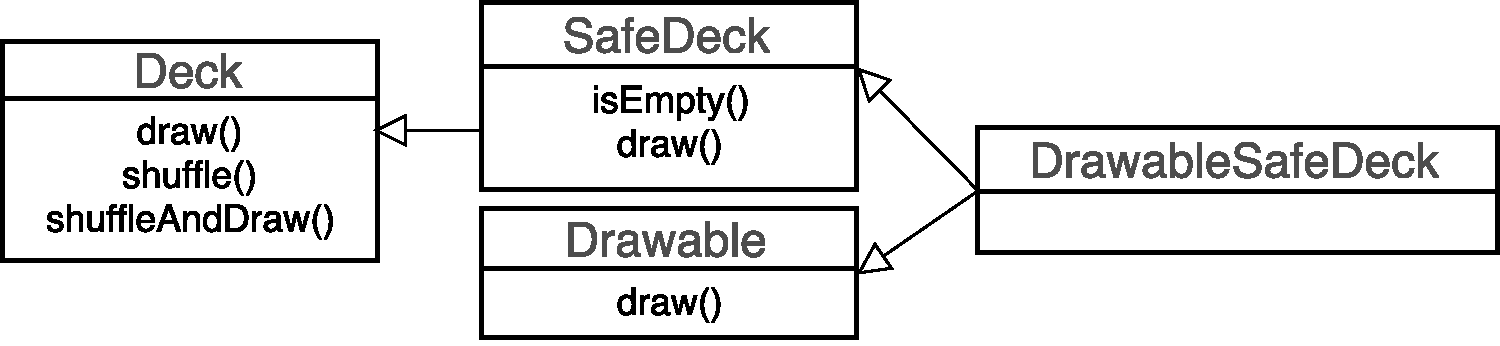
\includegraphics[height=2cm]{pics/DrawableSafeDeck.pdf}
% 	\caption{UML graph for \lstinline|DrawableSafeDeck|.}\label{fig:drawablesafedeck}
% 	\saveSpaceFig
% \end{figure*}

\begin{figure*}[t]
  % \nocaptionrule
  \centering
  \begin{minipage}[t]{0.28\textwidth}
  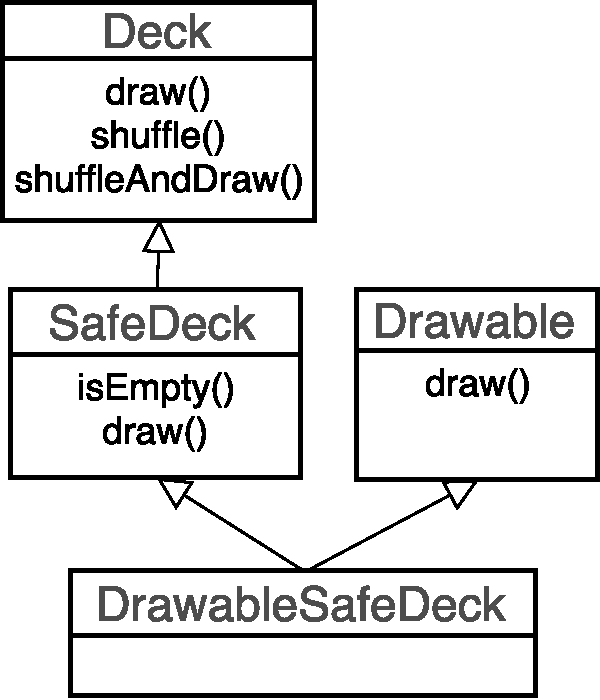
\includegraphics[height=4cm]{pics/DrawableSafeDeck1.pdf}
  \end{minipage}
  \centering
  \hspace*{2pt}
  \begin{minipage}[t]{0.4\textwidth}
  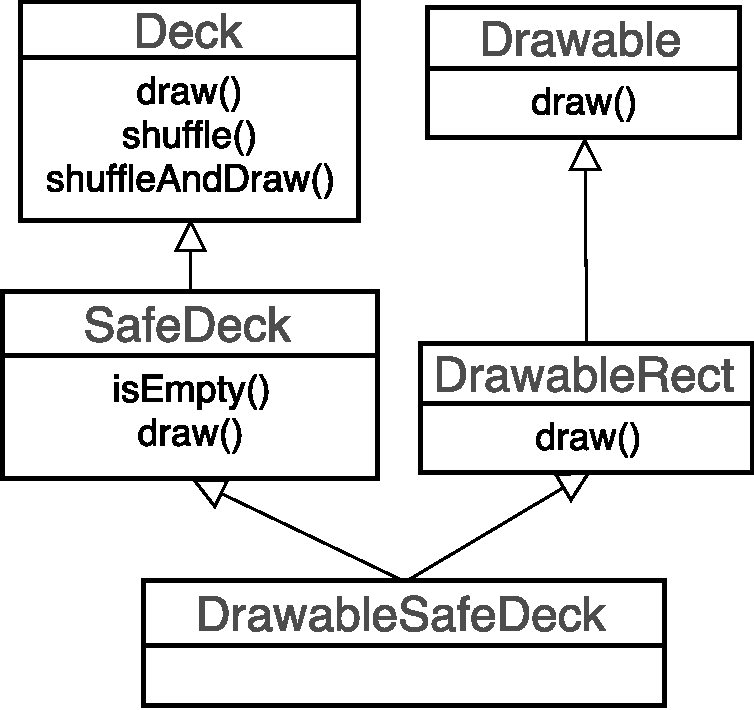
\includegraphics[height=4cm]{pics/DrawableSafeDeck0.pdf}
  \end{minipage}
  \centering
  \hspace*{2pt}
  \begin{minipage}[t]{0.25\textwidth}
  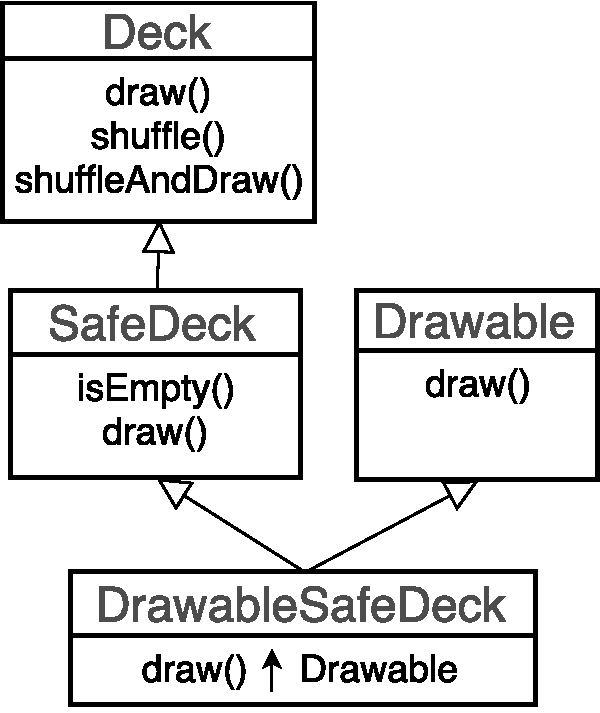
\includegraphics[height=4cm]{pics/DrawableSafeDeck3.pdf}
  \end{minipage}  
  \caption{UML graphs for \lstinline|DrawableSafeDeck|.}\label{fig:drawablesafedeck}
\end{figure*}
\yanlin{todo: change text and add a ref in Introduction}

\vspace{3pt}\begin{lstlisting}
interface DrawableSafeDeck extends Drawable, SafeDeck {}

// main program
new DrawableSafeDeck().shuffleAndDraw()
\end{lstlisting}\vspace{3pt}
When the \lstinline|DrawableSafeDeck| object calls \lstinline|shuffleAndDraw|, the implementation in \lstinline|Deck|
is dispatched. But then \lstinline|shuffleAndDraw| invokes ``\lstinline|this.draw()|'', and at this point, the receiver
is replaced by the object \lstinline|new DrawableSafeDeck()|.

From the perspective of \lstinline|DrawableSafeDeck|, the \lstinline|draw| method seems ambiguous. But ideally we would
like \lstinline|shuffleAndDraw| to invoke \lstinline|SafeDeck.draw|
because they belong to the same class hierarchy branch. It
seems that we choose dynamic dispatch but also make use of static type
information, since the type of this-reference (\lstinline|Deck|)
specifies the branch to use unambiguously.

%%\paragraph{Problem:} \\

\paragraph{\MIM's solution:} 
The essential problem is how to ensure that the correct method is
invoked. To solve this problem \MIM{} uses a variant of method
disptaching that we call \textit{hierarchical dispatch}. In
hierarchical dispatch both the static and dynamic type information 
ared used to select the right method implementation.
%Inspired by C++, we have formalized this feature into a minimal core calculus,
%studied and proved the type soundness. It is concise and can readily be imported to other systems. 
%And in the formalization, we propose \textit{hierarchical dispatch} in our model
%as the default method lookup algorithm. 
During the runtime, the method call \lstinline|e.m()|
makes use of both the static type and the dynamic type of the receiver, so it is seemingly a
combination of static and dynamic dispatch. Intuitively, the static type specifies one branch
to avoid ambiguity, and the dynamic type finds the most specific implementation on that branch. The formal algorithm will be introduced in Section~\ref{sec:formalization} and Section~\ref{sec:auxdefs}.

Using hierarchical dispatching the following code is accepted:
\vspace{3pt}\begin{lstlisting}
interface Deck {
  void draw() {...}
  void shuffle() {...}
  void shuffleAndDraw() { this.shuffle(); this.draw(); }
}
interface Drawable {...}
interface SafeDeck extends Deck {...}
interface DrawableSafeDeck extends Drawable, SafeDeck {}

// main program
new DrawableSafeDeck().shuffleAndDraw() // SafeDeck.draw is called
\end{lstlisting}\vspace{3pt}
During the runtime, when \lstinline|this.draw()| in called,
the dynamic type of the receiver is \lstinline|DrawableSafeDeck|, but the static type is actually
\lstinline|Deck|. Here it is an instance of the \textit{hierarchical invocation}, which can be read as 
``finding the most specific \lstinline|draw| along the path \lstinline|Deck|''. The meaning of ``along path
\lstinline|Deck|'' not only implies what \lstinline|Deck| inherits, but also the domain of its subtypes until the
dynamic type. Finally \lstinline|SafeDeck.draw| is correctly returned.

%Note that in C++, if we put the \lstinline[language=c++]|virtual| keyword in front of every \lstinline|draw| method, that means
%we enforce the dynamic dispatch, and it does the disambiguation correctly.
%Unfortunately, the C++ language, or rather the feature on triangle inheritance, has not been well formalized.

\paragraph{Implicit and Explicit Upcasts}
In our language model, there are two types of casts: \emph{implicit casts} and \emph{explicit upcasts}. The implicit casts appear
when passing arguments and returning expressions, they are also
upcasts. Hence all casts are safe. C++ implementations also support a
similar solution. However a notable difference between \MIM{} and C++
is that C++ checks ambiguity on casts, whereas our model is open to those safe casts. Unfortunately,
it introduces ambiguity in what we call ``the diamond inheritance'': when two methods override a same base method
but then accepted by multiple inheritance. The definition of such interfaces has to be rejected,
but this is natural as they are just two versions of the same operation, hence it is no longer an ``unintentional'' conflict.
Our proof demonstrates that it is a sufficient condition for type
soundness.
\bruno{I think the difference between C++ and our model is an important discussion, but very confusingly
  written. I believe that some more detail is needed. Do we have an
  extended discussion later?}




\subsection{Problem 3: Overriding on Individual Branches}\label{subsec:partialoverrides}

Method overriding is common in Object-Oriented Programming. 
With diamond inheritance where conflicting methods are intended to have 
the same semantics, method overriding is not a problem. If conflicting
methods arize from multiple parents, we can override all those methods 
in a single unified (or merged) method in the subclass. Therefore
further overriding is simple, because there is only one method that
can be overriden. 

With unintentional method conflicts, however, the situation is more
complicated because different, separate, conflicting methods can exist
in a class. Ideally we would like to support overriding for those
methods too, in exactly the same way that overriding is available for 
other (non-conflicting) methods. However we need to be able to
override the individual conflicting methods, rather than overriding all
conflicting methods into a single merged one. We illustrate the
problem and the need for a more refined overrding mechanism with 
an example.

Suppose that the programmer defines \lstinline|DrawableSafeDeck|, but he needs to override
\lstinline|Drawable.draw| and give a new implementation of drawing, so that the deck can indeed be visualized on the canvas.

%\paragraph{Problem:} how to update the conflicting methods separately, after the triangle inheritance.

\paragraph{Potential solutions/workarounds in existing languages:} Unfortunately in all languages we known
(including C++), the existing approaches are unsatisfactory.
One direction is to simply avoid this issue, by putting overriding before inheritance. For example, as shown in Figure~\ref{fig:drawablesafedeck}(right), we define a new component \lstinline|DrawableRect| that extends \lstinline|Drawable|, which simply draws the deck as a rectangle, and modifies the hierarchy:
\vspace{3pt}\begin{lstlisting}
interface DrawableRect extends Drawable {
  void draw() {
    JFrame frame = new JFrame("Canvas");
    frame.setSize(600, 600);
    frame.getContentPane().setBackground(Color.red);
    frame.getContentPane().add(new Square(10,10,100,100));
    ....
  }
}

interface DrawableSafeDeck extends DrawableRect, SafeDeck {}
\end{lstlisting} \vspace{3pt}
This workaround seems to work, but there are severe issues:
\begin{itemize}
	\item It changes the hierarchy and existing code, hence breaks the modularity.
	\item The demand for separate overriding after the triangle
          inheritance comes especially when there is
          interaction\bruno{what interaction?}. In the above code we assume
	that the overriding is unrelated to \lstinline|Deck|. But when the drawing relies on some information of the \lstinline|Deck|
	object, we have to either introduce field methods for delegation, or change the signature of \lstinline|draw| to take a parameter.
	Either way introduces unnecessary complexity and affects extensibility.
\end{itemize}

There are more involved workarounds in C++ using templates and complex
patterns, but such patterns are complex to use and there are still issues. A more detailed discussion of
such an approach is presented in Section~\ref{subsec:middleman}.

\paragraph{\MIM{}'s solution:} An additional feature of our model is \textit{hierarchical overriding}. It allows conflicting methods
to be overridden on individual branches, and hence offers independent extensibility. The above example can be easily realized by:
\vspace{3pt}\begin{lstlisting}
interface DrawableSafeDeck extends Drawable, SafeDeck {
  void draw() override Drawable {
    JFrame frame = new JFrame("Canvas");
    frame.setSize(600, 600);
    frame.getContentPane().setBackground(Color.red);
    frame.getContentPane().add(new Square(10,10,100,100));
    ...
  }
}

// main program
((Drawable)new DrawableSafeDeck()).draw(); // calls the latest draw
\end{lstlisting}\vspace{3pt}

Here the idea is that \emph{only} \lstinline{Drawable.draw} is
overriden. This is accomplished by specifying, in the method
definition, that only the method override only overrides the method 
from \lstinline|Drawable|.  
The direct support for individual overriding also works when there is interaction. In our formalization, this feature is necessary
and also involves in the algorithm of hierarchical dispatch.\bruno{the
last two sentences are a bit unclear. I think it is related to ``interaction''.}

\paragraph{Terminology:} The \lstinline|draw| methods we saw in
previous subsections\bruno{by now I saw many methods. Please be more precise.} are called \textit{original methods} in this paper, because they are originally defined in its interface.
In contrast, \lstinline|DrawableSafeDeck| defines a \textit{hierarchical overriding method}. The difference is that traditional method overriding overrides all branches by defining another original method, whereas hierarchical overriding only refines one branch.

\paragraph{A peek of hierarchical dispatching algorithm:} In our
model, triangle inheritance allows several original methods (branches)
to coexist, and hierarchical dispatch first finds the most specific
original method (branch), then it finds the most specific hierarchical
overriding on that branch. A quick counter-example is when there are
two hierarchical overriding methods on \lstinline|Drawable| in
\lstinline|DrawableSafeDeck|, it leads to ambiguity. The compiler is
supposed to forbid the case.\bruno{please show code illustrating this,
and improve explanation.}

A special rule for hierarchical overriding is: it can only refine \textbf{original} methods, and cannot jump over original methods with the same signature. For instance, writing \lstinline|"void draw()| \lstinline|override Deck {...}"| is disallowed in \lstinline|DrawableSafeDeck|, because existing two branches are \lstinline|Drawable.draw| and \lstinline|SafeDeck.draw|, while \lstinline|Deck.draw| is already covered. It does not really make sense to refine an old branch.

% Similar to many OO languages, the model also allows \textit{super method invocation} in a method body. The invocation \lstinline|super.T::m()| will ignore all the subtypes of \lstinline|T|, and only look at \lstinline|T| together with its super interfaces. It should behave the same as \lstinline|new T().m()| in principle.